
\chapter{Introduzione}
    \section{Obiettivi del sistema}
        L'obiettivo principale del sistema informatico DietiEstates25 e' la facilitazione della compravendita online di beni immobili sia per le agenzie immobiliare e gli agenti immobiliari che ci lavorano, che per i clienti. Gli agenti immobiliari saranno in grado di pubblicizzare gli immobili che desiderano vendere o affittare, e i clienti saranno in grado di visualizzarli e potenzialmente accordarsi con gli agenti per visitare o fare offerte sugli immobili.
    \section{Glossario}
    Sistema
    Agenzia Immobiliare
    Agente Immobiliare 
    Immobile
    Cliente
    Utente
    %Vendere
    %Affittare
    %Offerta
    %Amministratore
    Applicativo
    %Classe Energetica
    Inserzione
    API
    %Geoapify
    Dashboard
    Requisito
    %Requisito di Sistema
    %Requisito Utente
    %Requisito Funzionale
    %Requisito Non Funzionale
    %Requisito di Dominio
    Use Case
    %Fully-Dressed Use Case
    
\chapter{Specifica dei Requisiti}





    \section{Requisiti Utente}
        \subsection{Requisiti Funzionali}
            \begin{itemize}
                \item Ogni installazione di DietiEstates25 include un’utenza di amministrazione per il gestore
                dell’agenzia immobiliare, che viene creata con credenziali predefinite. Dopo aver effettuato
                l’accesso, è possibile modificare la password di amministrazione. L’amministratore può creare
                altri account di supporto all’amministrazione. I gestori di agenzie immobiliari possono a loro volta
                creare account per gli agenti immobiliari. Un utente interessato ai servizi immobiliari può
                registrarsi con un’e-mail e una password. È apprezzata la possibilità di effettuare la
                registrazione/login tramite credenziali di terze parti (e.g.: accedi con account Google, Facebook o
                GitHub). Gli utenti possono effettuare il login e accedere all’applicativo. Le credenziali devono
                essere salvate in modo sicuro.
                \item Gli agenti immobiliari possono caricare nuovi immobili con una serie di dettagli: foto, descrizione,
                prezzo, dimensioni, indirizzo, numero di stanze, piano, presenza di ascensore, classe energetica,
                ulteriori servizi presenti (portineria, climatizzazione, …), ecc. Gli immobili devono essere
                categorizzati in "vendita", "affitto". Forse in futuro sarà introdotto il supporto per affitti brevi e "case
                vacanze" (ma questa funzionalità al momento non è prevista). Ogni immobile inoltre è associato
                alla posizione geografica esatta, individuata interagendo con una mappa interattiva (tipo Google
                Maps).
                \item Gli utenti possono eseguire una ricerca avanzata di immobili con parametri multipli: tipologia di
                inserzione, prezzo minimo e massimo, numero di stanze, classe energetica, posizione, ecc. In
                particolare, deve essere possibile effettuare filtraggi per posizione geografica almeno al livello di
                comune o città. È apprezzata –ma non obbligatoria – la possibilità di effettuare ricerche di immobili
                che si trovano in un raggio arbitrario da un certo punto specificato dall’utente e selezionato su una
                mappa interattiva. La ricerca deve essere efficiente e performante. Gli immobili individuati nelle
                ricerche vengono visualizzati su una mappa interattiva (tipo Google Maps).
                \item I clienti devono poter prenotare una visita (nelle successive due settimane) per un immobile
                direttamente dal sistema. Gli agenti immobiliari ricevono notifiche (e-mail o interne al sistema, o
                possibilmente entrambe) quando una visita è prenotata per uno dei loro immobili. Le visite
                possono essere confermate o rifiutate dagli agenti. Se un appuntamento viene rifiutato, il cliente
                deve poter selezionare un altro orario. Sarebbe apprezzata la possibilità di integrare un calendario
                per gestire visivamente gli appuntamenti di un agente immobiliare.
                \item Gli utenti possono fare un’offerta su un immobile, specificando un prezzo eventualmente inferiore
                a quello riportato nell’inserzione. Gli agenti immobiliari possono accettare o rifiutare l'offerta, o
                fare una controproposta. Deve esserci un tracking delle offerte fatte e ricevute, magari uno storico
                visibile sia agli agenti sia ai clienti. Gli agenti hanno la possibilità di inserire manualmente offerte
                ricevute al di fuori del sistema.
                \item Quando viene creata un’inserzione, il sistema verifica automaticamente, tramite API di servizi
                esterni come Geoapify, la presenza di scuole, parchi pubblici, o fermate del trasporto pubblico nei
                pressi della posizione dell’immobile. Nel caso di riscontro affermativo, un apposito indicatore
                viene associato all’inserzione (“Vicino a scuole”, “Vicino a parchi”, “Vicina a trasporto pubblico”).
                \item Gli agenti immobiliari devono avere accesso a una dashboard con statistiche sugli immobili:
                numero di visualizzazioni dell’immobile, numero di visite prenotate, immobili venduti/affittati nel
                tempo, offerte ricevute, ecc. Deve essere possibile esportare report in formato PDF o Excel/CSV
                per la gestione interna delle agenzie.
                \item Gli utenti normali possono visualizzare un riepilogo delle attività svolte sul sito (immobili
                visualizzati, visite prenotate, offerte fatte).


            
        \end{itemize}
    \section{Requisiti di Sistema}
        \subsection{Use Case Diagram}
            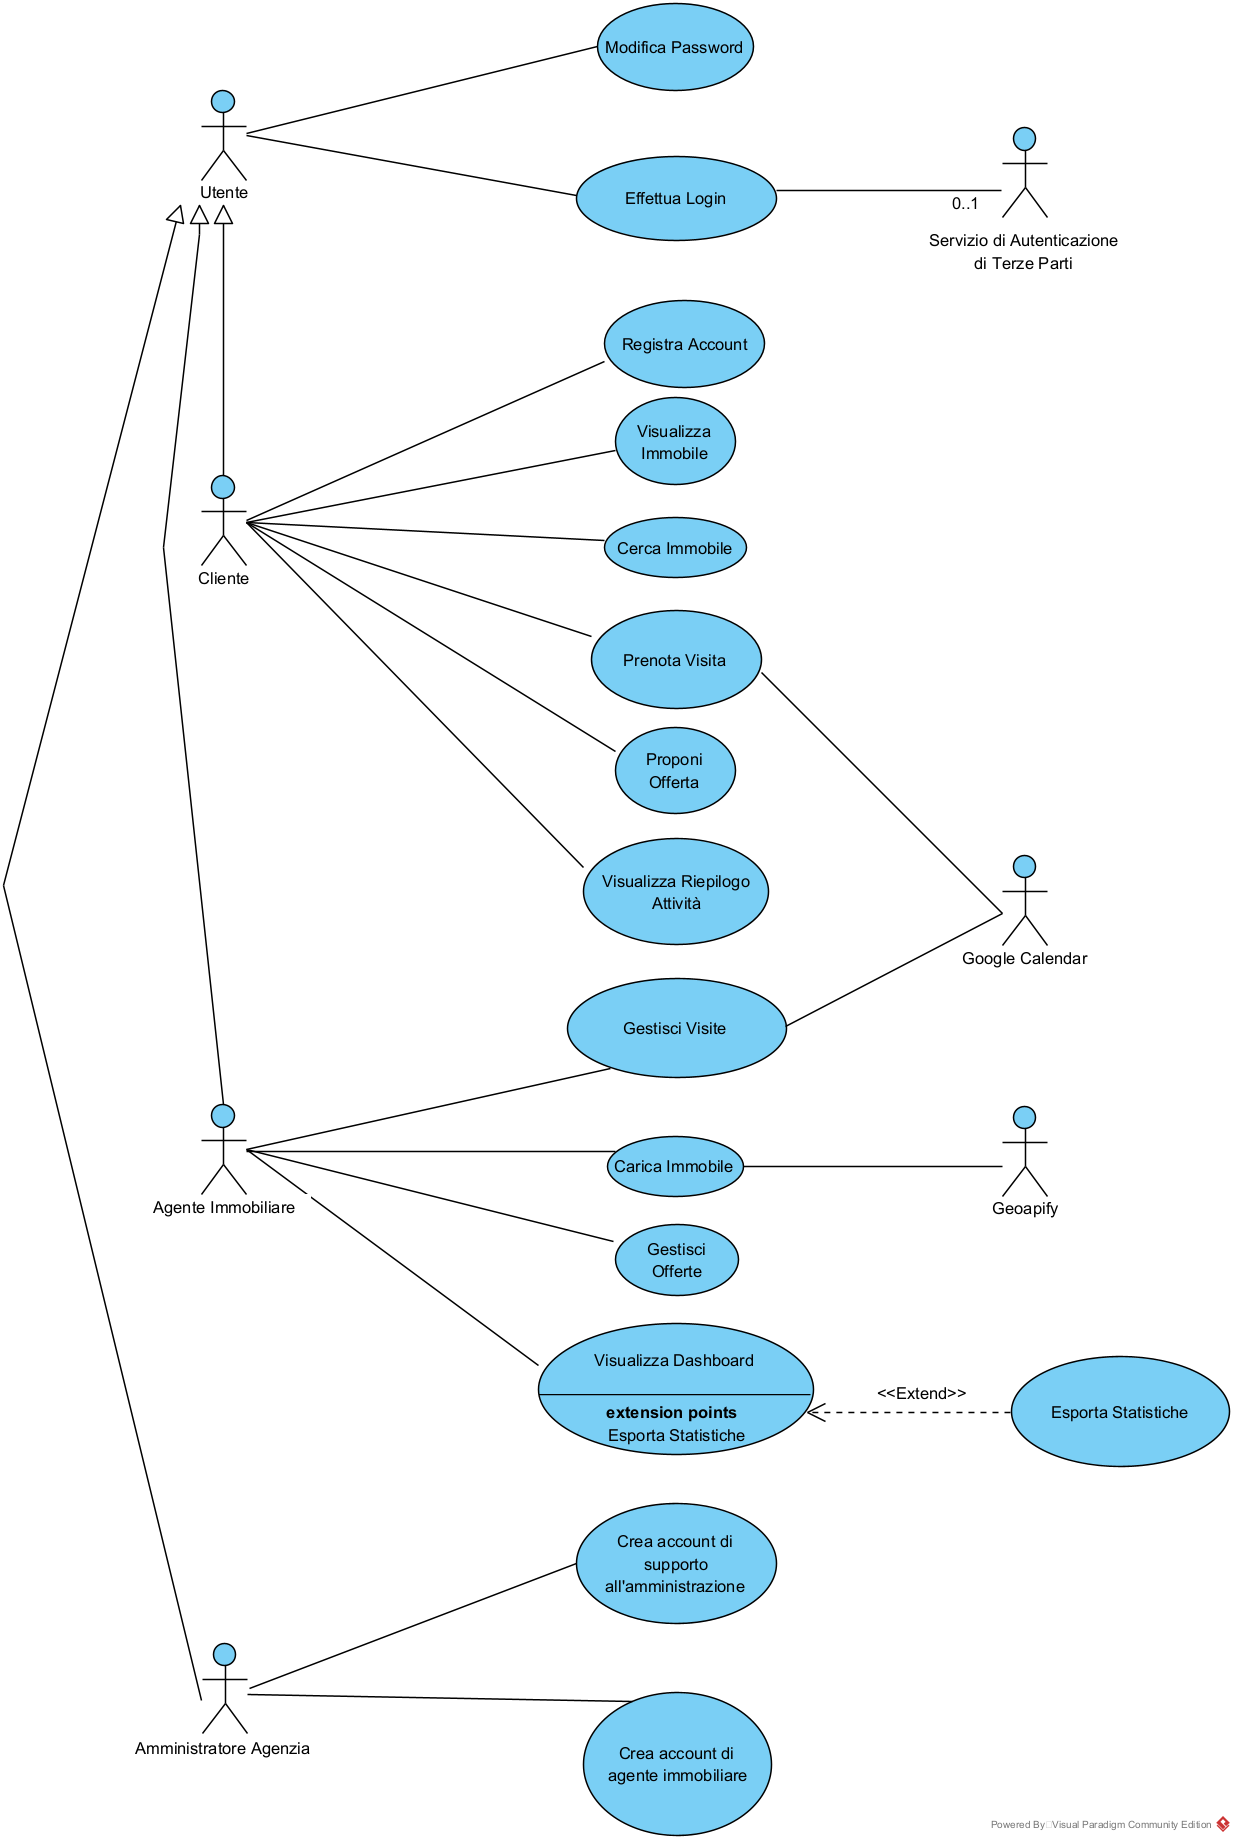
\includegraphics[width=\textwidth]{Immagini/Use Case Diagram Software Engineering Project 2024_25.png}
        \subsection{Fully Dressed Use Cases}
        %\begin{table}[htbp!]
    %\centering
    \begin{longtable}{|m{4cm}|m{4cm}|m{3cm}|m{4cm}|}
        \endfirsthead
        \hline
         & \textbf{Agente Immobiliare} & \textbf{Geoapify} & \textbf{Sistema} \\
        \hline
        \endhead % Intestazione che si ripete su tutte le pagine successive
        \hline
        \textbf{Nome Caso d'Uso} & \multicolumn{3}{p{11cm}|}{Carica Immobile} \\
        \hline
        \textbf{Goals in Context}
        & \multicolumn{3}{p{11cm}|}{L'agente immobiliare vuole caricare un nuovo immobile nel sistema} \\
        \hline
        \textbf{Preconditions}
        & \multicolumn{3}{p{11cm}|}{L'agente immobiliare deve essersi autenticato effettuando lo use case "Effettua Login"} \\
        \hline
        \textbf{Success End Condition}
        & \multicolumn{3}{p{11cm}|}{Il sistema tiene traccia dell'immobile caricato dall'agente immobiliare} \\
        \hline
        \textbf{Failed End Condition}
        & \multicolumn{3}{p{11cm}|}{Il sistema non tiene traccia dell'immobile caricato dall'agente immobiliare} \\
        \hline
        \textbf{Primary Actor}
        & \multicolumn{3}{p{11cm}|}{L'agente immobiliare} \\
        \hline
        \textbf{Trigger}
        & \multicolumn{3}{p{11cm}|}{L'agente immobiliare clicca sul pulsante "Crea Nuova Inserzione" della schermata M0} \\
        \hline

        \textbf{Main Scenario} & \textbf{Agente Immobiliare} & \textbf{Geoapify} & \textbf{Sistema} \\

        \hline
        \textbf{Step 1}& L'agente immobiliare clicca sul pulsante "Crea Nuova Inserzione" della schermata M0. & & \\
        \hline
        \textbf{Step 2}& & & Il sistema mostra la schermata M1. \\
        \hline
        \textbf{Step 3}& L'agente immobiliare seleziona la posizione geografica dell'immobile, riempe i campi e clicca sul pulsante "Step Successivo"  & & \\
        \hline
        \textbf{Step 4} & & & Il sistema mostra la schermata M2 \\
        \hline 
        \textbf{Step 5}& L'agente immobiliare riempe i campi e clicca sul pulsante "Step Successivo" & & \\
        \hline
        \textbf{Step 6}& & & Il sistema mostra la schermata M3 \\
        \hline 
        \textbf{Step 7} & L'agente immobiliare clicca sul pulsante "Carica Foto" e carica la foto che vuole caricare, poi clicca sul pulsante "Step Successivo" & & \\
        \hline
        \textbf{Step 8} & & & Il sistema mostra la schermata M4 \\
        \hline
        \textbf{Step 9}& L'agente immobiliare riempe i campi e clicca sul pulsante "Avanti" & & \\
        \hline
        \textbf{Step 10} & & & Il sistema mostra la schermata M5 \\
        \hline
        \textbf{Step 11} & L'Agente Immobiliare clicca sul pulsante "Conferma" & & \\
        \hline
        \textbf{Step 12} & & Geoapify verifica la presenza di zone d'interesse nei pressi dell'immobile e le segnala al sistema & \\
        \hline
        \textbf{Step 13} & & & Il sistema mostra la schermata M6 \\
        \hline
        \textbf{Step 14} & L'agente immobiliare clicca sul pulsante "Torna alla Home" & &  \\
        \hline
        \textbf{Step 15} & & & Il sistema tiene traccia dell'inserzione e mostra la schermata M0, terminando lo use case \\
        %\hline
    %\end{longtable}
    %\begin{longtable}{|m{4cm}|m{4cm}|m{3cm}|m{4cm}|}
    \hline
        \textbf{Extension 1:} \newline L'agente torna alla pagina precedente & & & \\
        \hline
        \textbf{Step 3a/5a/7a/9a/11a} & L'agente clicca sul pulsante "Step Precedente" o "Torna Indietro" & &  \\
        \hline
        \textbf{Step 4a/6a/8a/10a/12a} & & & Il sistema mostra la schermata precedente e si torna allo step 1/3/5/7/9 del Main Scenario ($M1 \to M0$, $M2 \to M1$, $M3 \to M2$, $M4 \to M3$, $M5 \to M4$) \\
        \hline
        \textbf{Extension 2:} \newline L'agente immobiliare aggiunge un tag descrittivo & & &  \\
        \hline
        \textbf{Step 5b} & L'agente immobiliare clicca sul pulsante '+' del tag che vuole aggiungere & & \\
        \hline
        \textbf{Step 6b} & & & Il sistema mostra il tag scelto dell'utente tra quelli inseriti e torna allo Step 5 del Main Scenario \\
        \hline
        \textbf{Extension 3:} \newline L'agente immobiliare rimuove un tag descrittivo & & & \\
        \hline
        \textbf{Step 5c} & L'agente immobiliare sposta il cursore sul tag e clicca sul pulsante "-" & & \\
        \hline
        \textbf{Step 6c} & & & Il sistema rimuove il tag dall'elenco e si ritorna allo Step 5 del Main  Scenario \\
        \hline
        \textbf{Extension 4:} \newline L'agente immobiliare rimuove una foto & & & \\
        \hline
        \textbf{Step 7d} & L'agente immobiliare sposta il cursore sulla foto e clicca sul pulsante "-" & & \\
        \hline
        \textbf{Step 8d} & & & Il sistema rimuove la foto dall'elenco e si ritorna allo Step 7 del Main Scenario \\
        \hline
        \textbf{Extension 5:} \newline L'agente immobiliare carica piú foto & & & \\
        \hline
        \textbf{Step 7e} & L'agente immobiliare clicca sul pulsante "Carica Foto" e carica la foto che vuole caricare & & \\
        \hline
        \textbf{Step 8e} & & & Si ritorna allo step 7 del Main Scenario \\
        \hline
    %\end{longtable}

    %\begin{longtable}{|m{4cm}|m{4cm}|m{3cm}|m{4cm}|}
    
    \end{longtable}
%\end{table}


\begin{longtable}{|m{4cm}|m{4cm}|m{3cm}|m{4cm}|}
        \hline
        \textbf{Nome Caso d'Uso} & \multicolumn{3}{p{11cm}|}{Prenota Visita} \\
        \hline
        \textbf{Goals in Context} & \multicolumn{3}{p{11cm}|}{Il cliente vuole prenotare una visita in presenza all'immobile} \\
        \hline
        \textbf{Preconditions}
        & \multicolumn{3}{p{11cm}|}{Il cliente deve essersi autenticato} \\
        \hline
        \textbf{Success End Condition}
        & \multicolumn{3}{p{11cm}|}{L'agente immobiliare che gestisce l'immobile viene notificato della richiesta di prenotazione} \\
        \hline
        \textbf{Failed End Condition}
        & \multicolumn{3}{p{11cm}|}{L'agente immobiliare che gestisce l'immobile non viene notificato della richiesta di prenotazione} \\
        \hline
        \textbf{Primary Actor}
        & \multicolumn{3}{p{11cm}|}{Cliente} \\
        \hline
        \textbf{Trigger}
        & \multicolumn{3}{p{11cm}|}{Il cliente clicca sul pulsante "Prenota Visita" della schermata M0} \\
        \hline

        \textbf{Main Scenario} & \textbf{Cliente} & \textbf{Google Calendar} & \textbf{Sistema} \\

        \hline
        \textbf{Step 1}& Il cliente clicca sul pulsante "Prenota Visita" della schermata M0 & & \\
        \hline
        \textbf{Step 2}& & & Il sistema mostra la schermata pop-up M1 \\
        \hline
        \textbf{Step 3}& Il cliente inserisce data e orario e clicca sul pulsante "Avanti" & & \\
        \hline
        \textbf{Step 4} & & & Il sistema mostra la schermata M2 \\
        \hline
        \textbf{Step 5} & Il cliente inserisce i suoi contatti e clicca sul pulsante "Avanti" & & \\
        \hline
        \textbf{Step 6} & & &Il sistema mostra la schermata M3\\ 
        \hline
        \textbf{Step 7} & Il cliente clicca sul pulsante "Conferma" & & \\
        \hline
        \textbf{Step 8} & & Google Calendar tiene traccia della richiesta di prenotazione e notifica l'agente immobiliare responsabile & \\
        \hline
        \textbf{Step 9} & & & Il sistema mostra la schermata M4 \\
        \hline
        \textbf{Step 10} & Il cliente clicca sul pulsante "Chiudi" & & \\
        \hline
        \textbf{Step 11} & & & Il sistema ritorna alla schermata M0 e termina il caso d'uso \\
        \hline
    \end{longtable}
    
\begin{longtable}{|m{4cm}|m{4cm}|m{3cm}|m{4cm}|}
    \hline
        \textbf{Extension 1:} \newline  Il cliente torna alla schermata precedente & & &\\
        \hline
        \textbf{Step 3a/5a/7a} & Il cliente clicca sul pulsante "Torna Indietro"& & \\
        \hline
        \textbf{Step 4a/6a/8a} & & & Il sistema mostra la schermata precedente e si torna allo step 1/3/5 del Main Scenario ($M1 \to M0$, $M2 \to M1$, $M3 \to M2$) \\
        \hline
        \textbf{Extension 2:} \newline Il cliente chiude la schermata pop-up & & &\\
        \hline
        \textbf{Step 3b/5b/7b/9b} & Il cliente chiude la schermata cliccando sulla "X" in alto a destra & &\\
        \hline
        \textbf{Step 4b,6b,8b,10b} & & & Il sistema mostra la schermata M0 e ritorna allo step 1 del Main Scenario \\
        \hline
    \end{longtable}
        \subsection{Mock-Up di Sistema}
        \subsection{Requisiti Non Funzionali}
            \begin{itemize}
                \item Il sistema dovrà essere raggiungibile al minimo per il 99,9\% del tempo.
                \item Il sistema dovrà essere un sistema distribuito composto da un front-end e un back-end indipendenti tra di loro, che comunicano tramite interfacce di programmazione accessibili via rete.
                \item Il sistema dovrà essere implementato usando esclusivamente linguaggi di programmazione Object Oriented.
                \item Il sistema dovrà essere performante.
        
            \end{itemize}


    

    \section{Personas}
    %\begin{table}[h!]
    %\centering
    \begin{tabular}{|m{6cm}|m{9cm}|}
    \hline
    \multicolumn{2}{|c|}{\textbf{Giacomo Murati}} \\
    \hline
    \centering \includegraphics[width=.25\textwidth]{Immagini/Giacomo Murati.jpg}
    & \textbf{Biografia}: Recentemente divorziato, urge trovare un nuovo appartamento il prima possibile. Laureato in architettura presso l'universita' Vanvitelli di Napoli. Disponibile e gentile, ma basta poco per farlo arrabbiare. È molto fiero del suo lavoro e delle sue conoscenze, ma questo lo porta a essere pieno di sé. Non ha un buon rapporto con i mezzi tecnologici, spesso lo irritano e infastidiscono. \\
    \hline
    \begin{tabular}{l} 
    \textbf{Età}: 59 \\
    \textbf{Locazione}: Napoli \\
    \textbf{Stato Civile}: Divorziato \\
    \textbf{Impiego}: Architetto \\
    \textbf{Tratti Personali}: Loquace, \\ Irascibile, Egocentrico
    \end{tabular}
    & \textbf{Goals}: Trovare un nuovo appartamento ben collegato in modo da poter visitare i figli e andare a lavoro. Data la sua professione, cerca una casa che soddisfi le sue esigenze e i suoi gusti estetici. \\
    \hline
    \end{tabular}
    \captionof{table}[Persona 1]{Persona 1}

    %\end{table}


    \begin{tabular}{|m{6cm}|m{9cm}|}
    \hline
    \multicolumn{2}{|c|}{\textbf{Juan Bandidos}} \\
    \hline
     \centering \includegraphics[width=.25\textwidth]{Immagini/Juan.jpg}
     & \textbf{Biografia}: Studente di Lettere presso una nota università portoghese. E' alla ricerca di un appartamento da fittare a breve termine per l'Erasmus che svolgera' in Italia il successivo anno scolastico. Ha iniziato a studiare la lingua italiana da poco e dunque ha ancora difficoltà a comprenderla. A causa di cio', ha gia' avuto problemi nella navigazione del sito web dell'università ospite. \\
    \hline
    \begin{tabular}{l} 
    \textbf{Età}: 20 \\
    \textbf{Locazione}: Lisbona \\
    \textbf{Stato Civile}: Single \\
    \textbf{Impiego}: Studente Universitario \\
    \textbf{Tratti Personali}: Insicuro, \\ Ipocondriaco, Curioso
    \end{tabular}
    & \textbf{Goals}: Trovare un appartamento da fittare durante la sua permanenza di 6 mesi. Preferirebbe che questo appartamento sia ben collegato all'universita'. \\
    \hline
    \end{tabular}
    \captionof{table}[Persona 2]{Persona 2}




    \begin{tabular}{|m{6cm}|m{9cm}|}
    \hline
    \multicolumn{2}{|c|}{\textbf{Gustavo Panini}} \\
    \hline
    \centering \includegraphics[width=.25\textwidth]{Immagini/Gustavo.jpg} 
    & \textbf{Biografia}: Erede dell'azienda del padre, Gustavo si e' rivelato un buon direttore che ha salvato l'azienda dalla rovina. Felicemente sposato da 20 anni, la sua famiglia comprende 3 figli, 4 cani e un pappagallo. La loro residenza attuale pero' non ha l'attrezzatura necessaria affinche' il figlio con disabilità possa vivere una vita tranquilla, e poiche' i figli stanno raggiungendo la fase adolescenziale, necessiteranno di piu' spazio nel prossimo futuro. \\
    \hline
    \begin{tabular}{l} 
    \textbf{Età}: 42 \\
    \textbf{Locazione}: Milano \\
        \textbf{Stato Civile}: Coniuge \\
    \textbf{Impiego}: Direttore di una \\ nota azienda multinazionale\\
    \textbf{Tratti Personali}: Caparbio, \\ Sicuro di se', Testardo
    \end{tabular}
    & \textbf{Goals}: Trovare una casa che possa soddisfare i bisogni della sua estesa famiglia, incluso il figlio il quale ha difficoltà motorie. \\
    \hline
    \end{tabular}
    \captionof{table}[Persona 3]{Persona 3}


    \begin{tabular}{|m{6cm}|m{9cm}|}
    \hline
    \multicolumn{2}{|c|}{\textbf{Rita Melograno}} \\
    \hline
    \centering \includegraphics[width=.25\textwidth]{Immagini/Agente imm.jpg}
    & \textbf{Biografia}: Lavora nel settore da 20 anni, ha sempre contattato clienti e venditori tramite chiamate cellulari. Costretta, controvoglia, dall'agenzia, ad adattarsi alle nuove tecnologie utilizzate nel settore, nonostante la poca esperienza ritiene che potra' apprenderle facilmente. Nel caso in cui non fosse in grado di apprenderle facilmente, sara' pronta a giudicare qualsiasi cosa che non le piaccia. Fin da giovane soffre di miopia e porta gli occhiali. \\
    \hline
    \begin{tabular}{l} 
    \textbf{Età}: 45 \\
    \textbf{Locazione}: Roma \\
        \textbf{Stato Civile}: Single \\
    \textbf{Impiego}: Agente immobiliare \\
    \textbf{Tratti Personali}: Piena di se', \\ Puntigliosa, Pigra
    \end{tabular}
    & \textbf{Goals}: Pubblicizzare gli immobili dei suoi clienti online \\
    \hline
    \end{tabular}
    \captionof{table}[Persona 4]{Persona 4}
    \subsection{Analisi delle Personas}
    Dopo aver analizzato le Personas, ci siamo resi conto di implementazioni aggiuntive necessarie al nostro sito. \newline
    Juan Bandidos, non avendo praticità con la lingua, ci ha fatto capire la necessità di un'interfaccia intuitivamente navigabile, anche senza che l'utente conosca perfettamente la lingua italiana. Abbiamo introdotto icone per facilitare la navigazione.\newline
    Inoltre, sempre grazie alla Persona di Juan Bandidos, abbiamo introdotto la possibilità di effettuare visite in remoto per gli immobili.\newline
    Queste aggiunte sono risultate molto importanti anche per la Persona di Rita Melograno, la quale, a causa di problemi di vista, trarrà beneficio sia dall'introduzione delle icone sia dalla grandezza delle scritte, non inferiore a 16 px.\newline
    Infine, grazie alla Persona di Gustavo Panini, prendendo in considerazione la necessità di attrezzature particolari dovute a difficoltà motorie, abbiamo reso obbligatorio un tag per specificare se un determinato immobile è dotato di strutture per disabili o meno, consentendo una ricerca mirata.\newline
\hfill



